% vim:spell spelllang=sk
\section{Gibbsov fenomén}
\label{section:gibbs}

V~príkladoch \ref{priklad:fourier_series_rect},
\ref{priklad:fourier_series_linear}
sme si ukázali Fourierove rady pre niektoré
nespojité funkcie. Táto kapitola bude venovaná ich spoločnej
vlastnosti - fenoménu "zvonenia" a~prestrelenia hodnoty funkcie 
v~blízkosti bodu nespojitosti. Zopakujme si grafy týchto dvoch príkladov.
\begin{priklad}
    Obdĺžniková funkcia
    \begin{equation*}
        f(x) = \left\{
            \begin{array}{l l}
                0 \quad x \in (-\pi,0) \\
                1 \quad x \in (0,\pi)
            \end{array}
        \right.
    \end{equation*}
    Jej $n$-tý čiastočný Fourierov súčet je
    \begin{equation*}
        S_n(x) = \frac{1}{2} + \frac{2}{\pi} \sum_{m=1}^{n}
                \frac{\sin\left( (2m-1) x\right)}{2m-1}, \quad n>0
    \end{equation*}

    Ukážka grafu čiastočných súčtov pre $n=10,100$ je na obrázku
    \ref{fig:gibbs_rect}.
    \begin{figure}[htp]
        \centering
        \subfigure[$n=10$]{
        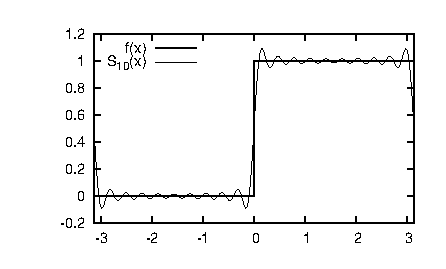
\includegraphics{obrazky/transformacia/gibbs/gibbs_saw10}
        }
        \subfigure[$n=100$]{
        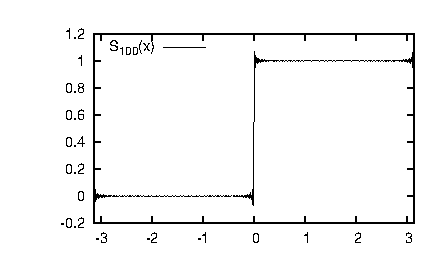
\includegraphics{obrazky/transformacia/gibbs/gibbs_saw100}
        }
        \caption{Ukážka Gibbsovho fenoménu na obdĺžnikovom signále}
        \label{fig:gibbs_rect}
    \end{figure}
    \label{priklad:gibbs_rect}
\end{priklad}
Môžeme si všimnúť zaujímavú vlastnosť, a~síce že čiastočné súčty
nemajú charakter konvergovať rovnomerne k~pôvodnej funkcii. Na druhú
stranu podľa \ref{veta:fourierova_veta} 
platí $S_n \imply f$ bodovo. V~praktickom slova
zmysle nám to hovorí, že čiastočné súčty síce konvergujú k~danej
funkcii, ale ich graf vykazuje isté nezrovnalosti. Jeho nepríjemnou
vlastnosťou je tendencia prestreliť hodnotu funkcie, a~to
nezanedbateľnou hodnotou, ako sa môžeme presvedčiť na príkladoch
\ref{priklad:gibbs_rect} a \ref{priklad:gibbs_linear}.

\begin{priklad}
    Uvažujme nasledujúcu funkciu:
    \begin{equation*}
        f(x) = \frac{1}{2} (\pi-x), \quad x\in(0,2\pi)
    \end{equation*}
    Jej čiastočný Fourierov súčet je
    \begin{equation*}
        S_n(x) = \sum_{k=1}^{n} \frac{\sin kx}{k}
    \end{equation*}
    ktorý sa dá odvodiť podobne ako riešenie príkladu
    \ref{priklad:fourier_series_linear}.
    Sľúbený graf pre hodnoty $n=10,100,1000$ sa nachádza na obrázku
    \ref{fig:gibbs_lin}.
    \begin{figure}[htp]
        \centering
        \subfigure[$n=10$]{
            \includegraphics{obrazky/transformacia/gibbs/gibbs_lin10}
        }
        \subfigure[$n=100$]{
            \includegraphics{obrazky/transformacia/gibbs/gibbs_lin100}
        }
        \subfigure[$n=1000$]{
            \includegraphics{obrazky/transformacia/gibbs/gibbs_lin1000}
        }
        \subfigure[$n=1000$, výrez]{
            \includegraphics{obrazky/transformacia/gibbs/gibbs_lin1000_2}
        }
        \caption{Gibbsov fenomén pre $f(x) = \frac{1}{2}(\pi-x)$}
        \label{fig:gibbs_lin}
    \end{figure}    
    \label{priklad:gibbs_linear}
\end{priklad}

Zvyšok tejto kapitoly venujeme práve tejto funkcii, jej čiastočným
súčtom a~odhadu o~koľko čiastočné súčty $S_n$ prestrelia hodnotu
$f(x)$. Príjemným výsledkom tohoto nášho snaženia bude záver pre
všetky funkcie $\in \PCab$.

\begin{lema}
    Funkcia $S_n(x)$ má na intervale $(0,\pi)$ extremálne body
    $\frac{2k}{n}\pi, \frac{2k+1}{n+1}\pi$ pre
    $k \in \{0,1,2,\dots,\floor{\frac{n-1}{2}} \}$
\end{lema}
\begin{dokaz}
    \begin{align*}
        S_n'(x) =& \sum_{k=1}^n \cos kx = 
            \frac{1}{2\sin(\frac{1}{2}x)} \sum_{k=1}^n 2
            \sin(\frac{1}{2}x) \cos(kx) =\\
            &=\frac{1}{2\sin(\frac{1}{2}x)} \sum_{k=1}^n
                \sin(\frac{1}{2}x + kx) +
                \sin(\frac{1}{2}x - kx) = \\
            &=\frac{1}{2\sin(\frac{1}{2}x)} \sum_{k=1}^n
                \sin(kx + \frac{1}{2}x ) -
                \sin(kx - \frac{1}{2}x ) = \\
            &=\frac{1}{2\sin(\frac{1}{2}x)} 
                \left(
                    \sin\left((n+\frac{1}{2})x\right) -
                    \sin(\frac{1}{2}x)
                \right) = \\
            &=\frac{ \sin(\frac{1}{2}nx) \cos(\frac{1}{2}(n+1)x)}
                {\sin(\frac{1}{2} x)}
    \end{align*}
    Na danom intervale je funkcia $\sin(\frac{1}{2} x)$ kladná a~preto
    extremálne body $S_n(x)$ sú nulové
    body $S_n'(x)$ a~to sú nulové body funkcií
     $\sin(\frac{1}{2}nx)$ a $\cos(\frac{1}{2}(n+1)x)$ čiže
     body
     $\frac{2 k \pi}{n},\, k\in \{1,\dots,\floor{\frac{n-1}{2}}\}$ a
     $\frac{(2k+1)\pi}{n+1},\, k\in
     \{0,1,\dots,..\floor{\frac{n-1}{2}}\}$. Zároveň však
     vieme, že pre body kde $\sin(\frac{1}{2} x)=0$ je
     $\cos(\frac{1}{2}(n+1)x)\not=0$ a~naopak.
     Preto $S_n'(x)$ v~týchto bodoch strieda znamienko a~teda to nie
     sú inflexné body $S_n$.
\end{dokaz}

\begin{lema}
    Funkcia $S_n(x)$ má na intervale $(0,\pi)$ maximá
    $\frac{2k+1}{n+1}\pi$ pre $ k \in \{0,1,2,\dots,\floor{\frac{1}{2}(n-1)} \}$
    a~minimá
    $\frac{2k}{n}\pi, $ pre
    $k \in \{1,2,\dots,\floor{\frac{1}{2}(n-1)} \}$
\end{lema}
\begin{dokaz}
    Platí
    \begin{equation*}
        \frac{2k}{n}\pi < \frac{2k+1}{n+1}\pi < \frac{2(k+1)}{n} \pi,
        \quad k \in \{1,2,\dots,\floor{\frac{n-1}{2}} \}
    \end{equation*}
    a~tiež
    \begin{equation*}
        \frac{2k+1}{n+1}\pi < \frac{2k+2}{n}\pi < \frac{2k+3}{n+1} \pi,
        \quad k \in\{1,2,\dots,\floor{\frac{n-1}{2}}-1 \}
    \end{equation*}
    Teda, dané dve postupnosti bodov sa striedajú. Využitím výsledku
    predchádzajúcej lemy a~uvážením, že extremálne body sa striedajú,
    máme výsledok na dosah. Stačí dokázať, že bod $\frac{1}{n+1}\pi$
    je maximom $S_n(x)$. To je ale zrejmé, lebo
     $S_n'(x)$ je kladná na intervale $(0, \frac{1}{n+1}\pi)$.
\end{dokaz}

\begin{definicia}[Sinc funkcia]
    Nenormalizovanou funkciou $\sinc t$ nazveme funkciu
    \begin{equation*}
        \sinc(t) = \left\{
            \begin{array}{l l}
                \frac{\sin t}{t}, \quad& t\not=0\\
                1,\quad&t=0
            \end{array}
            \right.
    \end{equation*}
    Okrem nenormalizovanej funkcie $\sinc t$ existuje aj takzvaná
    normalizovaná funkcia $\sinc' y = \sinc \pi y$. V~tejto publikácii
    budeme až na zdôraznené výnimky používať nenormalizovanú definíciu.
\end{definicia}

\begin{veta}
Pre každé $s\in\N$, postupnosť
$\left\{S_n\left( \frac{2s-1}{n+1}\pi\right)\right\}_{n=1}^{\infty}$
má limitu $\int_0^{(2s-1)\pi} \sinc t \dd t$. Podobne, postupnosť
$\left\{S_n\left( \frac{2s}{n}\pi\right)\right\}_{n=1}^{\infty}$
má limitu $\int_0^{2s\pi} \sinc t \dd t$.
\end{veta}

\begin{dokaz}
    \begin{equation}
        \begin{split}
        S_n\left(\frac{2s-1}{n+1}\pi\right) &=
            \sum_{k=1}^n \frac{1}{k}
            \sin\left(\frac{k(2s-1)}{n+1}\pi\right) \\
            &=
         \frac{2s-1}{n+1}\pi    
            \sum_{k=1}^n \frac{n+1}{k(2s-1)\pi}
            \sin\left(\frac{k(2s-1)}{n+1}\pi\right) \\
            &=
         \frac{2s-1}{n+1}\pi    
            \sum_{k=1}^n \sinc\left( \frac{k(2s-1)}{n+1} \pi \right)            
        \end{split}
        \label{eq:gibbs_convergence}
    \end{equation}
    Na druhú stranu, zoberme si Riemannov horný a~dolný
    integrálny súčet funkcie $\sinc t$ na intervale $(0,L)$.
    Uvažujme rovnomerné rozdelenie intervalu na $n$ rovnakých častí.
    Potom $H_n \ge \frac{L}{n} \sum_{k=0}^{n-1} \sinc(\frac{k L}{n}) \ge D_n$
    ako sa môžeme ľahko presvedčiť.
    Porovnaním s \eqref{eq:gibbs_convergence} a~uvážením faktu
    $\sinc 0 =1$ dostávame
    \begin{equation*}
        H_{n+1} \ge S_n\left(\frac{2s-1}{n+1}\pi\right) +
        \frac{2s-1}{n+1}\pi \ge D_{n+1}
    \end{equation*}
    Následne
    \begin{equation*}
        \begin{split}
       \int_0^{2s-1} \sinc t \dd t &= 
       \limtoinf{n} H_{n+1} - \frac{2s-1}{n+1}\pi \ge 
       \limtoinf{n} S_n\left(\frac{2s-1}{n+1}\pi\right) \ge \\
       &\ge
       \limtoinf{n} D_{n+1} - \frac{2s-1}{n+1}\pi =
       \int_0^{2s-1} \sinc t \dd t                     
      \end{split}
    \end{equation*}
    Analogicky ukážeme aj druhú nerovnosť    
\end{dokaz}

Označme $G(x) = \frac{2}{\pi} \int_0^{\pi x} \sinc t \dd t$.
Keďže pre ľubovoľné $s\in N$, $\limtoinf{n} \frac{1}{2} (\pi -
\frac{2s-1}{n+1} )=\frac{\pi}{2}$, môžeme hovoriť, že
$n$-tý čiastočný súčet prestrelí hodnotu funkcie
v~svojom $k$-tom maxime $G(2k-1)$ krát ak
$n$ pošleme do nekonečna.
Funkciu $G(k)$ môžete vidieť na obrázku \ref{fig:gibbs_sincint}.

\begin{figure}[htp]
    \centering
    \includegraphics{obrazky/transformacia/gibbs/sincintegral}
    \caption{Integrál funkcie $\sinc x$}
    \label{fig:gibbs_sincint}
\end{figure}


Tabelované hodnoty pre prvých niekoľko miním a~maxím môžeme nájsť 
v~tabuľke \ref{tab:gibbs_table}. 

\begin{table}[htb]
    \centering
    \begin{tabular}{c|c|c|c|c|c|}
        k&1&2&3&4&5 \\ \hline
        Minimá &0.90282&0.94994&0.96641&0.97475&0.97978 \\
        Maximá &1.17898&1.06619&1.04021&1.02883&1.02246
    \end{tabular}
    \caption{Tabelované hodnoty miním a maxím funkcie $G(x) =
    \frac{2}{\pi} \int_0^{\pi x} \sinc t \dd t$}
    \label{tab:gibbs_table}
\end{table}

Z~hodnôt je zrejmé, že čiastočné súčty prestrelia funkciu takmer 
o~18\%, čo je prekvapivo veľa. Ak by sme počítali túto hodnotu nie
vzhľadom na aktuálnu hodnotu $f(x)$ ale vzhľadom na veľkosť skoku,
táto hodnota bude polovičná. 

Kapitolu zavŕšime zovšeobecnením
\begin{veta}
    Nech $f,f'\in\PC(0,2\pi)$. Nech $S_n$ je $n$-tý čiastočný súčet.
    Potom graf $S_n$ konverguje k~náčrtu na obrázku
    \ref{fig:gibbs_figura}.
    Na obrázku je $a$ všeobecný bod nespojitosti funkcie $f$.
    Vertikálny rozdiel je 
    $\frac{2}{\pi} |\lim_{x\imply a^+} f(x) - \lim_{x\imply a^-} f(x)|
    \int_0^{\pi} \sinc t \dd t$ a~je
    centrovaná okolo 
    $\frac{1}{2}(\lim_{x\imply a^+} f(x) + \lim_{x\imply a^-} f(x))$
\end{veta}
\begin{dokaz}
    Nebudeme uvádzať. Zvedavý čitateľ ho môže nájsť v \cite{hewitt},
    kde sa taktiež môže dočítať viac o~Gibbsovom fenoméne, jeho
    histórii a~nájde užitočné odkazy na ďalšiu literatúru.
\end{dokaz}

\begin{figure}[htp]
    \centering
    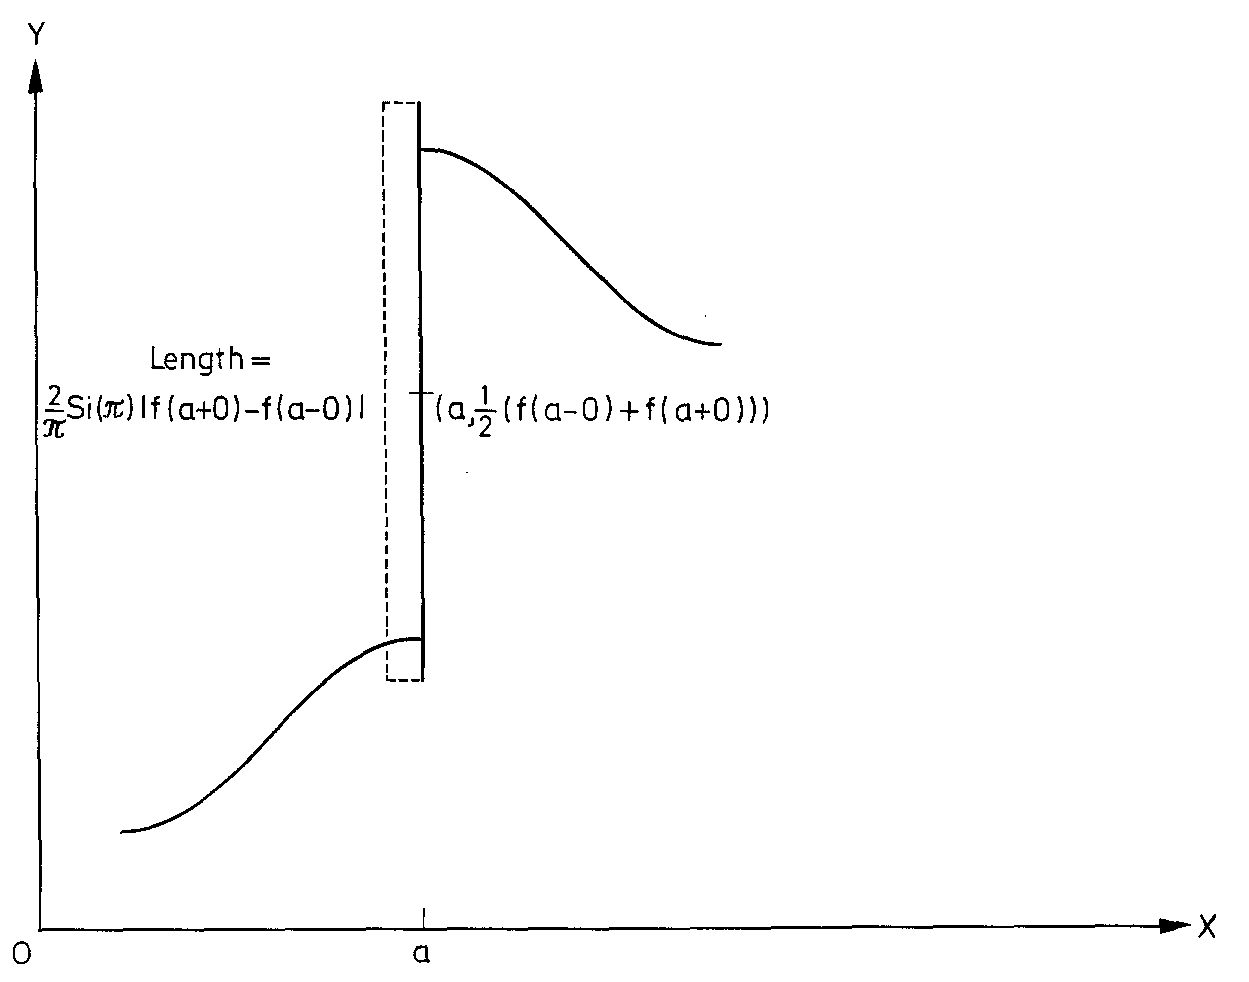
\includegraphics[width=10cm]{obrazky/transformacia/gibbs/gibbs_figura}
    \label{fig:gibbs_figura}
    \caption{Náčrt Gibbsovho fenoménu vo všeobecnosti}
\end{figure}
